\documentclass[a4paper,titlepage,10pt]{article}

\usepackage[T1]{fontenc}
\usepackage[utf8]{inputenc}
\usepackage{polski}

\usepackage{enumerate}
\usepackage{amssymb}
\usepackage{amsmath}
\usepackage[pdftex]{graphicx}
\usepackage{tikz}
\usepackage[colorlinks=true,linkcolor=blue]{hyperref}

\usepackage[a4paper, top=2.5cm, bottom=2.5cm]{geometry}
\linespread{1.3}

\title{\huge Symulacja układu planetarnego na GPU\\ przy użyciu CUDA i OpenGL\\\small Dokumentacja biznesowa}
\author{Daniel Kłobuszewski\and Jakub Kotur}

\begin{document}
	\maketitle

	\section{Wstęp}\label{sec:wstep}
	
	\paragraph{}

\begin{figure}[h]
	\centering
	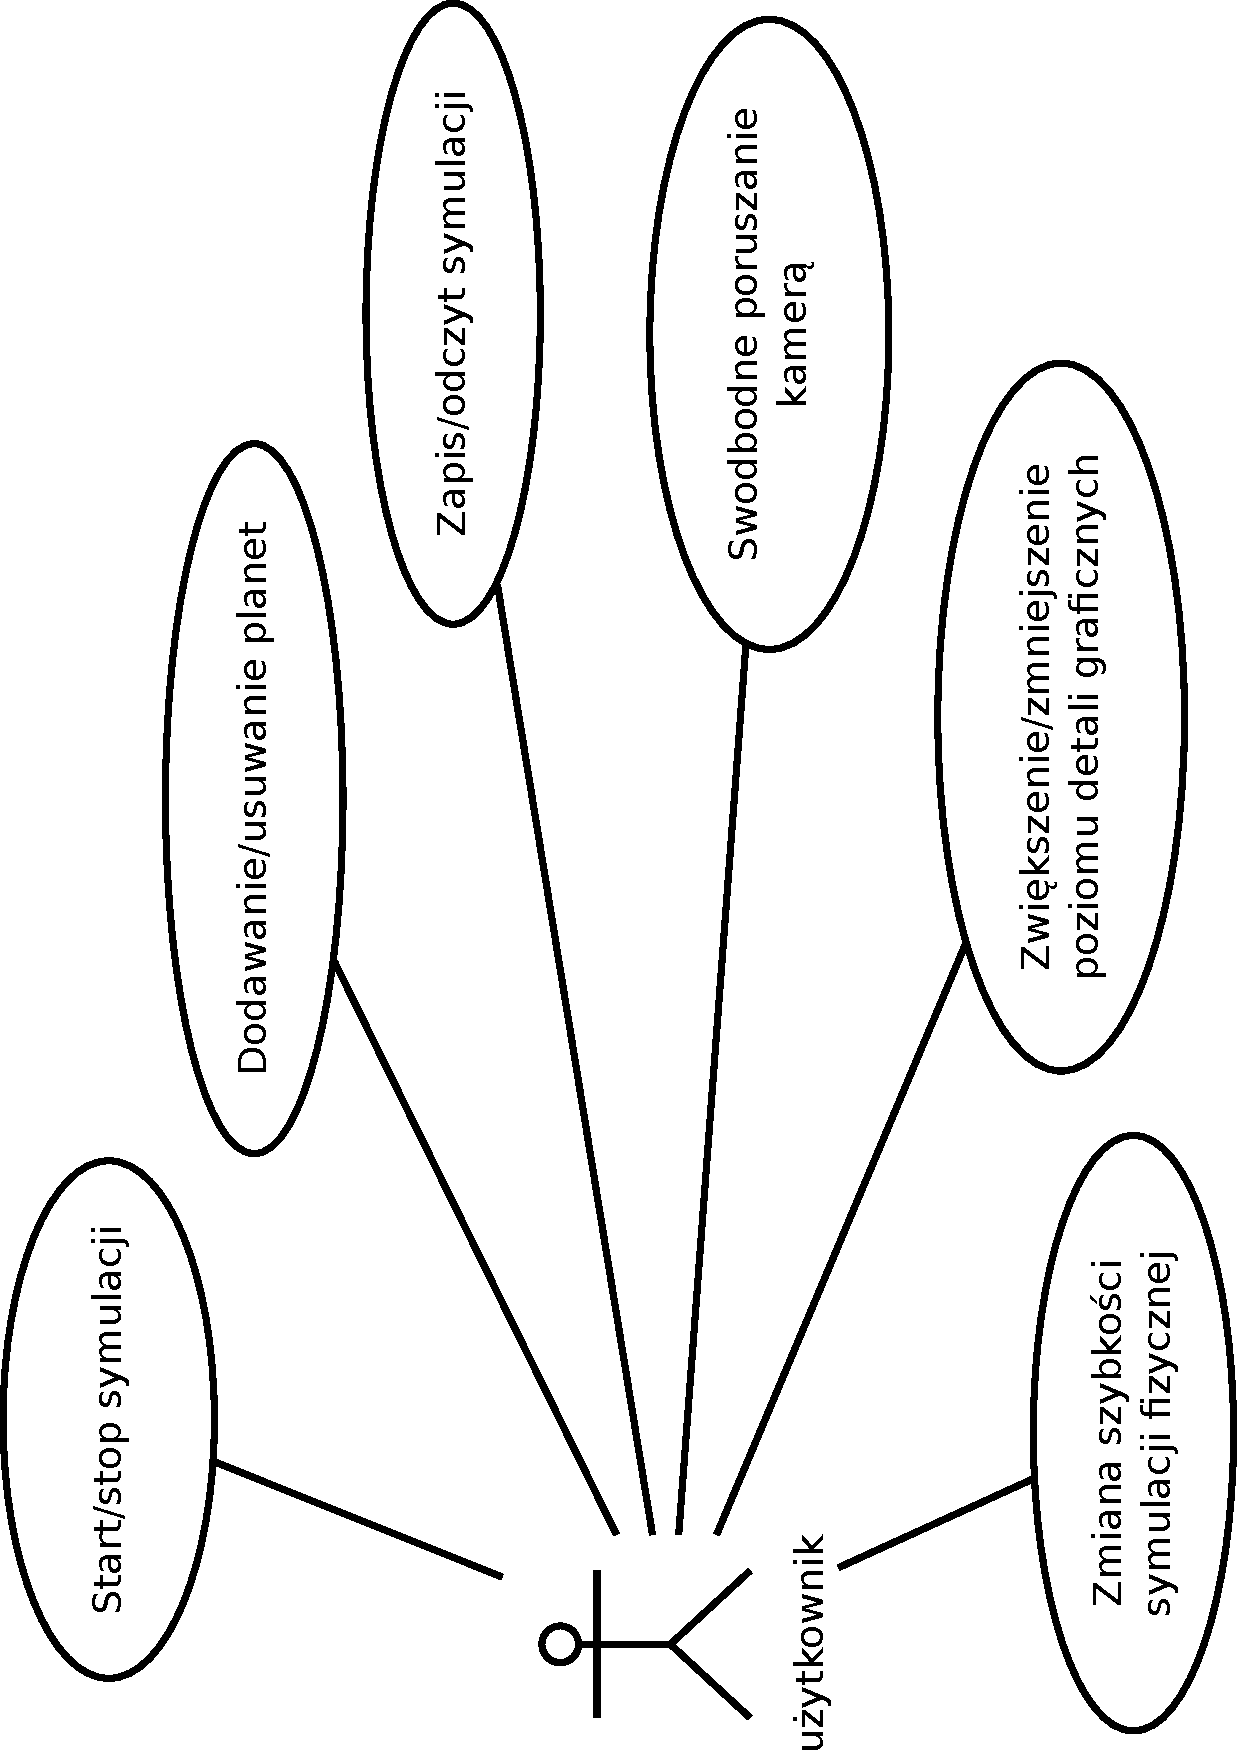
\includegraphics[width=0.7\textwidth,angle=-90]{use-case.pdf}
	\caption{Diagram przypadków użycia}
	\label{fig:use-case}
\end{figure}

\end{document}

